%% ---------------------------------------------------------------------------
%%  side.tex -- summary of the work: problem, prior work, method, what was
%%  tried, results, novelty, status, next steps.  pdflatex side && pdflatex side
%%  Every number is taken from paper/main.tex or fidings/divergence_investigation.md.
%% ---------------------------------------------------------------------------
\documentclass[10pt,twocolumn,a4paper]{article}
\usepackage[margin=1.7cm,columnsep=0.6cm]{geometry}
\usepackage{amsmath,amssymb}
\usepackage{graphicx}
\graphicspath{{./}{paper/}}
\usepackage{booktabs}
\usepackage{tabularx}
\usepackage{xcolor}
\usepackage{tikz}
\usetikzlibrary{arrows.meta,positioning,calc}
\usepackage{enumitem}
\setlist{itemsep=1pt,topsep=2pt,leftmargin=12pt}
\usepackage[hidelinks]{hyperref}
\usepackage{titlesec}
\titleformat{\section}{\large\bfseries}{\thesection}{0.6em}{}
\titlespacing*{\section}{0pt}{9pt}{3pt}
\titlespacing*{\subsection}{0pt}{6pt}{2pt}
\usepackage{caption}
\captionsetup{font=small,labelfont=bf}

\definecolor{acc}{HTML}{A85A0A}
\definecolor{accbg}{HTML}{F6E9D6}
\definecolor{fail}{HTML}{7A2E6E}
\definecolor{soft}{HTML}{EDEFF1}
\definecolor{fed}{HTML}{E8EEF3}

\tikzset{
  box/.style ={draw, rectangle, rounded corners=1.5pt, align=center, inner sep=3pt,
               font=\footnotesize, fill=white},
  inp/.style ={box, fill=soft},
  new/.style ={box, draw=acc, line width=0.8pt, fill=accbg},
  ar/.style  ={-{Stealth[length=4pt]}, line width=0.5pt},
  aracc/.style={ar, draw=acc, line width=0.8pt},
}

\title{\textbf{Phase-Relational \texorpdfstring{$Q$}{Q}-Learning}\\[3pt]
\large One traffic light controller for every intersection:\\
the problem, the work done, the results and the current status}
\author{Author Name}
\date{September 2026}

\begin{document}
\maketitle

% =============================================================================
\section{The problem}
Reinforcement learning can control traffic lights well at the intersection it was
trained on. A city, however, would want something different: a controller trained
once on a few intersections that can then be installed at new intersections, in new
parts of the city, without being trained again. This is called zero-shot transfer
across intersection topologies.

We train one shared neural network for all intersections of several cities, using
federated learning, so each city trains locally and only model weights are exchanged.
The goal is that this single network also works on a road network none of the cities
trained on. For a long time it did not: on unseen networks it caused gridlock. The work
explains why, fixes it, and tests the fix.

% =============================================================================
\section{Why it is hard: the phase numbering problem}

\subsection{Explained simply}
Imagine several street crossings, each with a panel of buttons that change the lights.
On the first crossing, button 1 lets cars turn left. On the second crossing, button 1
lets cars go straight. A robot that learns from both crossings tries to remember
``button 1 is a good idea when many cars wait'', and becomes confused, because button 1
does something different in each place. At a new crossing it cannot know what button 1
does.

A better robot ignores button numbers. Each button carries a label saying what it does,
for example ``lets 12 waiting cars turn left''. The robot learns to read the labels, and
the labels mean the same thing at every crossing, including new ones.

\subsection{Stated formally}
Intersection $i$ has $A_i$ signal phases, and $A_i$ ranges from 2 to 8 in our networks.
A shared $Q$ network must output a fixed number of values, so the usual design pads the
output to $A_{\max}$ and masks unused actions:
\[
Q_\theta(o_i)=W\,h_\theta(o_i)+b,\qquad
a_i=\arg\max_{k:\,m_i[k]=1} Q_\theta(o_i)[k].
\]
Row $W_k$ alone values ``action $k$'' at every intersection. But the order of phases in a
signal program is chosen by whoever built the network. In the four RESCO benchmark
networks we use, phase 1 is a protected left turn in two networks and a through movement
in the other two. Row $W_1$ is trained on contradictory targets and learns nothing that
carries over to a new network. A second possible cause is that when an unseen network
has more phases than any training city, some rows are never trained at all. These two
causes need different fixes, so we tested them separately.

% =============================================================================
\section{What already exists}
Avoiding phase numbers is not a new idea. Table~\ref{tab:prior} lists the closest work
and how ours relates to it.

\begin{table}[ht]
\centering\footnotesize
\setlength{\tabcolsep}{3pt}
\begin{tabularx}{\columnwidth}{@{}p{18.5mm}X@{}}
\toprule
Work & Idea, and relation to ours \\
\midrule
FRAP (2019) & Scores phases through pairs of competing movements. Needs a hand written
table mapping each intersection's phases to movements before it can control it. We
ported it and use it as a baseline. \\
MPLight (2020) & FRAP with pressure as state and reward, scaled to thousands of
signals. Needs the same table. \\
AttendLight (2020) & Attention over lanes and phases, one model for many intersection
types; its authors note it generalises when similar configurations appear in
training. \\
TransferLight (2024) & Zero-shot control on unseen road networks, credited to training
on many random networks. Not yet compared with ours. \\
HFRL (2025) & Federated signal control that clusters intersections before averaging.
Federated, but not about transfer to unseen topologies. \\
Braun (2026) & Concurrent work: a graph network scores movements, and the method builds
its own phase sets in place of the network's signal program. We ran its code on our
networks (Section~\ref{sec:results}). \\
RESCO (2021) & The benchmark whose networks and published results we use. \\
\bottomrule
\end{tabularx}
\caption{Closest prior and concurrent work.}
\label{tab:prior}
\end{table}

% =============================================================================
\begin{figure*}[t]
\centering
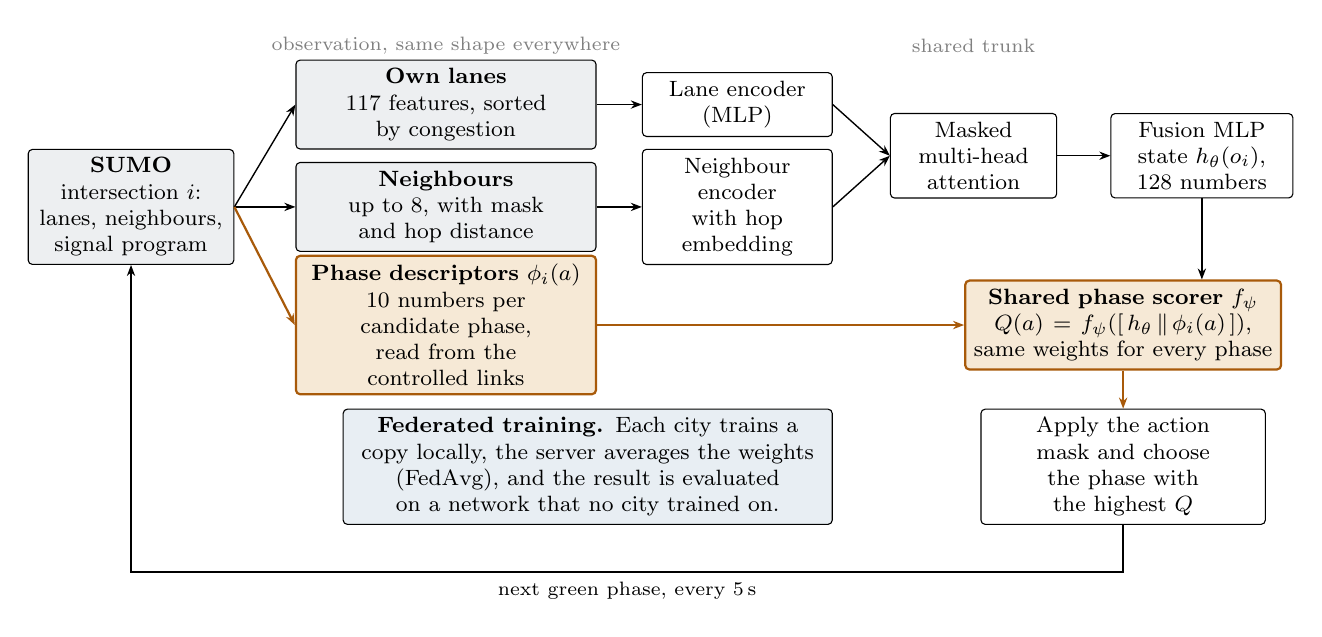
\begin{tikzpicture}[x=1mm,y=1mm]
\node[inp, text width=24mm] (sumo) at (14,3) {\textbf{SUMO}\\ intersection $i$:\\ lanes, neighbours,\\ signal program};
\node[inp, text width=36mm] (own) at (54,16) {\textbf{Own lanes}\\ 117 features, sorted by congestion};
\node[inp, text width=36mm] (nbr) at (54,3) {\textbf{Neighbours}\\ up to 8, with mask and hop distance};
\node[new, text width=36mm] (phi) at (54,-12) {\textbf{Phase descriptors} $\phi_i(a)$\\ 10 numbers per candidate phase,\\ read from the controlled links};
\draw[ar] (sumo.east) -- (own.west);
\draw[ar] (sumo.east) -- (nbr.west);
\draw[aracc] (sumo.east) -- (phi.west);
\node[box, text width=22mm] (lenc) at (91,16) {Lane encoder\\ (MLP)};
\node[box, text width=22mm] (nenc) at (91,3) {Neighbour encoder\\ with hop embedding};
\node[box, text width=19mm] (att) at (121,9.5) {Masked multi-head\\ attention};
\node[box, text width=21mm] (fus) at (150,9.5) {Fusion MLP\\ state $h_\theta(o_i)$,\\ 128 numbers};
\draw[ar] (own.east) -- (lenc.west);
\draw[ar] (nbr.east) -- (nenc.west);
\draw[ar] (lenc.east) -- (att.west);
\draw[ar] (nenc.east) -- (att.west);
\draw[ar] (att.east) -- (fus.west);
\node[new, text width=38mm] (score) at (140,-12) {\textbf{Shared phase scorer} $f_\psi$\\ $Q(a)=f_\psi([\,h_\theta\,\|\,\phi_i(a)\,])$,\\ same weights for every phase};
\node[box, text width=34mm] (arg) at (140,-30) {Apply the action mask and choose\\ the phase with the highest $Q$};
\draw[aracc] (phi.east) -- (score.west);
\draw[ar] (fus.south) -- (fus.south |- score.north);
\draw[aracc] (score.south) -- (arg.north);
\draw[ar] (arg.south) -- ++(0,-6) -| node[pos=0.25,below,font=\scriptsize]{next green phase, every 5\,s} (sumo.south);
\node[box, fill=fed, text width=60mm] (fed) at (72,-30) {\textbf{Federated training.} Each city trains
  a copy locally, the server averages the weights (FedAvg), and the result is
  evaluated on a network that no city trained on.};
\node[font=\scriptsize,gray] at (54,23.5) {observation, same shape everywhere};
\node[font=\scriptsize,gray] at (121,23.5) {shared trunk};
\end{tikzpicture}
\caption{The model. Every intersection produces an observation of the same shape, so one
network serves all of them without knowing which city it is in. The highlighted parts
are the phase-relational readout: each candidate phase is described by what it does,
and one shared scorer rates it.}
\label{fig:model}
\end{figure*}

% =============================================================================
\section{What we did}
We replaced the numbered output layer with a scorer that rates each candidate phase from
a description of what it does (Figure~\ref{fig:model}):
\[
Q_\theta(o_i)[a]=f_\psi\big([\,h_\theta(o_i)\,\|\,\phi_i(a)\,]\big),
\qquad \phi_i(a)\in\mathbb{R}^{10}.
\]
The descriptor $\phi_i(a)$ contains the phase's pressure (incoming minus outgoing queue),
its queue, waiting time, occupancy and lane count, whether it is currently shown and for
how long, and the share of its green lanes that go straight, left and right. It is
computed automatically from the simulator, so a new intersection needs no manual setup.
The number of parameters no longer depends on the number of phases, so there are no
untrained rows and no indices whose meaning can conflict. Because the descriptor includes
per phase pressure, the classic max pressure rule is also inside what the model can
represent.

Training is federated across three RESCO networks (arterial4x4, cologne3, ingolstadt7),
and the model is evaluated on grid4x4, which no city trains on. All experiments use the
SUMO simulator.

% =============================================================================
\section{What we tried along the way}
The fix came at the end of a long investigation, recorded in a dated lab notebook of 110
sections.
\begin{itemize}
\item \textbf{The symptom.} Trained policies often collapsed into a confident, repetitive
      behaviour that gave the same reward on 30 different traffic seeds. Removing
      federation did not change this, so federation was not the cause.
\item \textbf{Measurement problems.} We found six evaluation errors, each of which had
      produced a believable but wrong number. For example, the evaluator silently tested on
      a training city when shapes did not match, and our simulator settings used a 2\,s
      yellow instead of the benchmark's 3\,s, giving every controller more green time. One
      earlier claim was withdrawn because of this.
\item \textbf{41 interventions} that kept the numbered output: other aggregation rules and
      clustering, larger or different architectures, other algorithms (PPO, QR-DQN, CQL,
      MAML, evolution strategies), reward shaping, curricula, and fine tuning on the new
      network. 32 gave nothing or made things worse, 4 were unclear and 5 helped. None fixed
      the transfer failure.
\item \textbf{The representation.} We then suspected the numbering itself, tested it
      against the untrained rows explanation, and introduced the phase-relational readout.
\end{itemize}

% =============================================================================
\section{What we achieved}\label{sec:results}
All results use six random seeds unless stated. A difference counts as significant when
$|\Delta|/\mathrm{SE}\ge 2$. Delay is computed only over vehicles that arrive, so the share
of trips completed is always given next to it.

\paragraph{The cause is the numbering.}
On a test network where every row of the numbered output is fully trained, the numbered
output still gridlocks: reward $-9028.88$, against $-9296.84$ when untrained rows are
present. The difference is within seed noise. This control experiment is the central
result.

\paragraph{Transfer to an unseen network.}
The phase-relational readout outperforms the numbered output by four orders of magnitude
on five different configurations, with all six seeds agreeing ($|\Delta|/\mathrm{SE}$ from
23.6 to 96.7). Table~\ref{tab:zs} shows the two configurations that use the benchmark's
own settings.

\begin{table}[ht]
\centering\footnotesize
\setlength{\tabcolsep}{4pt}
\begin{tabular}{@{}llrr@{}}
\toprule
Setting & Controller & Reward & Trips done \\
\midrule
fully RESCO & Numbered output & $-8965.09$ & 19.5\% \\
matched & \textbf{Phase-relational} & $\mathbf{-0.16}$ & \textbf{98.9\%} \\
RESCO & Numbered output & $-9705.49$ & 16.4\% \\
timing & \textbf{Phase-relational} & $\mathbf{-0.20}$ & \textbf{98.8\%} \\
same network & Max pressure & $-0.380$ & 99.2\% \\
 & Fixed time & $-2.730$ & 97.7\% \\
\bottomrule
\end{tabular}
\caption{Unseen network (grid4x4), final training round. Higher reward is better. The
numbered output completes only 16 to 20\% of trips.}
\label{tab:zs}
\end{table}

\paragraph{Against max pressure,} a strong hand designed controller, on the unseen network:
lower waiting time on all six seeds (18.8\,s against 22.8\,s), with the same share of trips
completed (98.8\% against 99.2\%). On average delay the two are tied (41.4\,s against
40.2\,s).

\paragraph{Against FRAP.} Given its hand written table for every network, FRAP also
transfers, which confirms the explanation independently. Our readout reaches the same
level without the table: better on the best round for all six seeds, while the final
round difference is not significant.

\paragraph{On RESCO's Cologne scenario,} trained on three cities at the same time, the
policy reaches 21.4\,s average delay with 91.6\% of trips completed. Max pressure gives
22.4\,s at 98.6\%, and RESCO's published learned methods give 22.13\,s (IPPO) and 23.99\,s
(IDQN), without reported completion rates. We describe this as comparable performance.
On Ingolstadt, max pressure is better (26.6\,s against 35.2\,s).

\paragraph{Against the concurrent method (Braun 2026),} run from its released code and
measured the same way: on the unseen network, 293\,s average delay (94.4\% of trips done)
against our 41.4\,s (98.8\%). It is also behind ours on Cologne and Ingolstadt. His method
was designed for throughput and for other networks, so this is a comparison on our
benchmark only.

\paragraph{Earlier results, explained.} We repeated the two strongest of the 41
interventions with the new readout. Both stopped helping: plain averaging now beats the
curriculum on all six seeds, and fine tuning on the new network, previously the largest
gain, now makes the policy slightly worse. This suggests the earlier experiments were
limited by the numbering, rather than showing that those ideas do not work.

% =============================================================================
\section{What is new}
\begin{itemize}
\item \textbf{A control experiment that identifies the cause.} Earlier phase based methods
      replaced the numbered output without measuring why it fails. We show that the
      failure remains when every row is trained, which rules out the simpler explanation
      and the cheap fixes it suggests.
\item \textbf{Phase descriptors built automatically} from the simulator. No intersection
      needs a hand written table, unlike FRAP and MPLight, and the network's own signal
      program is kept, unlike Braun's method.
\item \textbf{A new reading of 41 negative results}, supported by two measured reversals.
\item \textbf{Six evaluation pitfalls}, three of which come from common tooling.
\end{itemize}
What is \emph{not} new: phase based scoring itself (FRAP, AttendLight), zero-shot transfer
across networks (TransferLight), and federated signal control (HFRL).

% =============================================================================
\section{Current status}
\begin{itemize}
\item A complete paper draft in IEEE format: 10 pages, 31 checked references.
\item Confirmed with six seeds: the control experiment, transfer on five configurations,
      the comparison with max pressure, the training budget test, the FRAP comparison,
      both reversals, and a test showing that adding more varied training networks does
      not help.
\item Screens with three seeds: the comparison with Braun's method (its six seed training
      finishes today, evaluation follows) and an ensemble of models.
\item All code, run histories and the lab notebook are kept, and every number in the paper
      has been re-derived from raw data.
\end{itemize}

% =============================================================================
\section{Open questions and next steps}
\paragraph{Is it ready to submit?} The central claim is well supported. The cause is
isolated by a control experiment, the fix holds on five configurations with six seeds, it
is tested at the benchmark's own settings, and it is checked against an independent method
(FRAP) and a concurrent one (Braun). What a reviewer is most likely to ask for:
\begin{itemize}
\item a direct comparison with TransferLight;
\item more than four real networks, including a real city network;
\item longer training budgets, closer to published practice;
\item an explanation of the tie with max pressure on delay.
\end{itemize}

\paragraph{Possible future work.}
\begin{itemize}
\item A reward that targets delay rather than waiting, since the policy wins on the
      quantity it is trained on and ties on the other.
\item Adapting to real rather than synthetic traffic on a new network.
\item Testing why FRAP does worse on corridor networks. Our data suggest it depends on how
      many movements have a downstream lane in the model, and Braun reports a similar
      sensitivity.
\item Larger and more varied networks, and eventually a real deployment study.
\end{itemize}

\paragraph{Where it could go.} The draft is written as a method and evaluation paper
rather than a performance paper. A transportation venue would value the configuration
free controller and the RESCO results. A machine learning venue focused on benchmarks or
methodology would value the control experiment and the evaluation pitfalls. A conference
version would need to be shorter, while a journal could keep all experiments.

\end{document}
